\documentclass[conference]{IEEEtran}
\IEEEoverridecommandlockouts
% ----------------------------------------------------------------------------
% Editing Guidelines for AI Agents and Contributors
% ----------------------------------------------------------------------------
% Please preserve the formatting and structure of this template.
%
% Rules:
% 1. Do not modify the document class, packages, or custom commands unless
%    explicitly requested.
%
% 2. Preserve the order of sections and subsections. Do not rename, remove,
%    or reorder them unless instructed.
%
% 3. After every completed section, subsection, figure, table, placeholder,
%    abstract, keywords block, or other major block, always insert:
%
%       \vspace{\baselineskip}
%
%    to maintain consistent vertical spacing throughout the document.
%
% 4. Separate logical blocks (paragraphs, sections, figures, tables, lists,
%    etc.) with one empty source line to keep the .tex file clean and readable.
%
% 5. Keep indentation and formatting consistent with the existing template.
%    Avoid unnecessary whitespace or formatting changes.
%
% 6. Preserve labels (\label{}), citations (\cite{}), references,
%    captions, and bibliography entries. Never rename labels unless every
%    corresponding reference is also updated.
%
% 7. Do not remove comments, placeholders, or explanatory notes unless they
%    are explicitly replaced by finalized content.
%
% 8. When adding figures or tables:
%       - Always include \caption{} and \label{}.
%       - Place \label{} immediately after \caption{}.
%       - Add \vspace{\baselineskip} after the environment.
%
% 9. Do not manually change margins, font sizes, spacing, or page layout.
%    Follow IEEEtran formatting at all times.
%
% 10. Keep the source code organized so that future edits produce the minimum
%     possible diff (avoid reformatting unrelated lines).
% ---------------------------------------------------------------------------

% ----------------------------------------------------------------------------
% Packages
% ----------------------------------------------------------------------------
\usepackage{cite}
\usepackage{amsmath,amssymb,amsfonts}
\usepackage{algorithmic}
\usepackage{graphicx}
\usepackage{textcomp}
\usepackage{xcolor}
\usepackage[utf8]{inputenc}
\usepackage[T1]{fontenc}
\usepackage[most]{tcolorbox}
\usepackage[colorlinks=true, urlcolor=blue]{hyperref}

% ----------------------------------------------------------------------------
% Commands
% ----------------------------------------------------------------------------
\newcommand{\placeholder}[1]{\colorbox{yellow}{\parbox{\dimexpr\linewidth-2\fboxsep}{#1}}}
\newcommand{\email}[1]{\underline{\textcolor{blue}{#1}}}

% ----------------------------------------------------------------------------
% Fixes
% ----------------------------------------------------------------------------
\def\BibTeX{{\rm B\kern-.05em{\sc i\kern-.025em b}\kern-.08em
    T\kern-.1667em\lower.7ex\hbox{E}\kern-.125emX}}

\makeatletter
\renewenvironment{abstract}
{
  \par\small
  \noindent\textbf{Abstract}---\normalfont
}
{\par}
\makeatother
\makeatletter
\renewenvironment{IEEEkeywords}
{
  \par\small
  \noindent\textbf{Keywords}---\normalfont
}
{\par}
\makeatother

\renewcommand{\IEEEkeywordsname}{\textbf{Keywords}}
% ----------------------------------------------------------------------------
% Document
% ----------------------------------------------------------------------------
\begin{document}

% ----------------------------------------------------------------------------
% Title and Authors
% ----------------------------------------------------------------------------
\title{Estrategia Integral de Pruebas de Software en Focalboard: Un Enfoque de Pruebas Unitarias, Funcionales, de Integración y Sistema\\}

\author{
\IEEEauthorblockN{
Marco Antonio Marquez Herrera,
Ricardo Mauricio Chambilla Perca,
Alejandro Sebastian Alfonso Huacasi, \\
Daniel Wilston Chura Monroy,
Gabriela Vanessa Martell Villanueva,
Jeferson Jofre Quispe Madariaga
}

\IEEEauthorblockA{
\text{Escuela Profesional de Ingeniería de Sistemas} \\
\text{Universidad Nacional de San Agustín}\\
{\color{blue}\underline{mmarquezhe@unsa.edu.pe}}, {\color{blue}\underline{rchambillap@unsa.edu.pe}},
{\color{blue}\underline{aalfonso@unsa.edu.pe}},\\
{\color{blue}\underline{dchuramo@unsa.edu.pe}},
{\color{blue}\underline{gmartellv@unsa.edu.pe}},
{\color{blue}\underline{jquispemad@unsa.edu.pe}}}
}

% ----------------------------------------------------------------------------
% Abstract
% ----------------------------------------------------------------------------
\maketitle

\begin{abstract}
Focalboard es una herramienta de gestión de proyectos que integra una aplicación web en React y TypeScript, un servidor en Go, una API REST, comunicación WebSocket y una capa de persistencia compatible con distintos motores de base de datos. En este trabajo se presenta la estrategia de pruebas aplicada a la versión 8.0.0 del sistema. Para ello se combinaron pruebas unitarias, funcionales, de integración y de sistema. Las pruebas unitarias se ejecutaron con Go testing y Jest; los casos funcionales se diseñaron mediante técnicas de caja negra; la integración se verificó en diez flujos críticos; y las pruebas de sistema evaluaron seguridad y usabilidad mediante Cypress. La automatización se implementó con GitHub Actions y SonarQube Cloud. Se diseñaron 106 casos funcionales, de los cuales 97 fueron ejecutados: 80 resultaron exitosos, 17 no exitosos y 9 quedaron pendientes por restricciones del entorno. Los 56 casos de integración y los dos escenarios de sistema seleccionados finalizaron correctamente. El análisis estático informó 71.4\% de cobertura global, valor inferior al criterio inicial de 85\%. Los resultados muestran que la estrategia permite reproducir las verificaciones principales y detectar tanto defectos funcionales como deuda de pruebas. También evidencia que una ejecución exitosa no reemplaza el análisis del alcance ni la revisión del Quality Gate.
\end{abstract}
\vspace{\baselineskip}

% ----------------------------------------------------------------------------
% Keywords
% ----------------------------------------------------------------------------
\begin{IEEEkeywords}
pruebas de software, cobertura de código, pruebas de integración, Cypress, integración continua, Focalboard
\end{IEEEkeywords}
\vspace{\baselineskip}

% ----------------------------------------------------------------------------
% Introduction
% ----------------------------------------------------------------------------
\section{Introducción}
Focalboard permite organizar trabajo mediante tableros, tarjetas, propiedades y distintas vistas. Su edición personal combina varios componentes: la interfaz ejecuta acciones en el navegador, el servidor valida permisos y reglas, la capa de aplicación coordina los cambios y el almacenamiento conserva el estado. Por ello, probar una función únicamente desde una capa no permite observar todos los errores que pueden aparecer durante su uso.

En este artículo se presenta la estrategia aplicada para evaluar Focalboard. El propósito fue relacionar requisitos funcionales con casos verificables, completar pruebas para las APIs críticas y automatizar su ejecución. El trabajo consideró cuatro niveles: unitario, funcional, integración y sistema. El modelo de calidad ISO/IEC 25010:2023 sirvió para delimitar los atributos de sistema \cite{iso25010}. El énfasis se puso en comparar lo que cada nivel puede detectar y en registrar resultados reales, incluso cuando no alcanzaron el criterio propuesto.

El resto del artículo está organizado de la siguiente manera: en las Secciones II y III se describen el sistema y los requisitos; en las Secciones IV a VIII se presentan la estrategia y las pruebas; en la Sección IX se explica la automatización; y finalmente se discuten los resultados, conclusiones y trabajos futuros.
\vspace{\baselineskip}

% ----------------------------------------------------------------------------
% System Description
% ----------------------------------------------------------------------------
\section{Descripción del sistema}

% --- Subsection: Context and Purpose ---
\subsection{Contexto y propósito de Focalboard}
Focalboard es una herramienta de código abierto, multilingüe y autoalojada para definir, organizar y seguir el trabajo de personas y equipos. El proyecto dispone de una edición de escritorio para un usuario y una edición de servidor multiusuario \cite{focalboardRepo}. En este trabajo se evaluó la versión 8.0.0 del repositorio, con énfasis en la edición de servidor y su aplicación web.
\vspace{\baselineskip}

% --- Subsection: General Architecture ---
\subsection{Arquitectura general de la aplicación}
La aplicación sigue una arquitectura cliente-servidor por capas. La interfaz React utiliza \texttt{octoClient} para comunicarse con la API REST. Los manejadores de \texttt{server/api} delegan las operaciones en \texttt{server/app}; esta capa aplica reglas de negocio y accede a la interfaz \texttt{Store}. Las implementaciones SQL permiten trabajar con SQLite, PostgreSQL y MySQL. En paralelo, \texttt{server/ws} distribuye cambios de tableros y bloques a los clientes conectados. La Fig.~\ref{fig:arquitectura_general} resume este recorrido.

Una operación típica comienza cuando el usuario modifica una tarjeta. El frontend transforma la acción en una solicitud HTTP; el manejador recupera la sesión, verifica permisos y valida el cuerpo antes de llamar a la aplicación. Si la escritura termina correctamente, el servidor devuelve la representación actualizada y difunde un evento. Los demás clientes reciben el mensaje y actualizan su estado sin recargar la página. Esta secuencia justificó que las pruebas de integración observaran no solo la respuesta, sino también los cambios persistidos y las notificaciones producidas.

\begin{figure}[htbp]
\centering
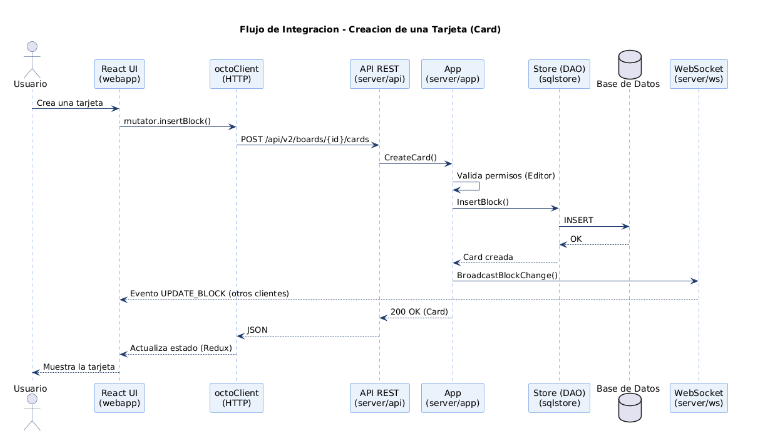
\includegraphics[width=\columnwidth]{../../docs/images/img5.png}
\caption{Arquitectura general de Focalboard.}
\label{fig:arquitectura_general}
\end{figure}
\vspace{\baselineskip}

% --- Subsection: Technology Stack ---
\subsection{Stack tecnológico}
El backend utiliza Go 1.21, \texttt{gorilla/mux} para el enrutamiento y \texttt{gorilla/websocket} para la comunicación en tiempo real. El frontend emplea TypeScript 4.6, React 17, Redux Toolkit y Webpack 5. Las pruebas se apoyan en Go testing, Testify, Jest 27 y Cypress 9. La persistencia admite SQLite, PostgreSQL, MySQL y MariaDB dentro de la matriz de CI. Docker permitió reproducir en Windows el entorno Linux requerido por el servidor de pruebas.

La selección de herramientas siguió la tecnología de cada capa. Go testing pertenece al entorno estándar del servidor y Testify proporciona aserciones legibles. Jest trabaja sobre los archivos TypeScript transformados por SWC y Testing Library permite verificar componentes desde elementos visibles. Cypress controla un navegador y ejecuta acciones semejantes a las de un usuario. Finalmente, GitHub Actions coordina estos comandos en runners limpios, evitando que una ejecución dependa de archivos o procesos conservados en una computadora local.
\vspace{\baselineskip}

% --- Subsection: Components Selected for Testing ---
\subsection{Componentes seleccionados para las pruebas}
Se seleccionaron autenticación, tableros, tarjetas y bloques, miembros y permisos, categorías, búsqueda, importación y exportación, suscripciones, WebSocket y persistencia. La elección responde a tres razones: concentran las operaciones de mayor uso, conectan más de una capa y contienen decisiones de acceso o conservación de datos. De esta manera, una misma función pudo observarse desde una unidad aislada, una API y un flujo completo.
\vspace{\baselineskip}

% ----------------------------------------------------------------------------
% Functional Requirements Evaluated
% ----------------------------------------------------------------------------
\section{Requisitos funcionales evaluados}

% --- Subsection: Identification of Functional Requirements ---
\subsection{Identificación de requisitos funcionales}
Los requisitos se obtuvieron del catálogo elaborado a partir de las rutas REST, los modelos, la interfaz y la documentación del repositorio. El catálogo contiene dieciséis grupos, desde RF-001, gestión de acceso y autenticación, hasta RF-016, auditoría y cumplimiento. Cada requisito se contrastó con una operación observable; por ejemplo, RF-004 se relacionó con crear, editar, duplicar y eliminar tableros, mientras RF-008 se relacionó con crear y modificar tarjetas.
\vspace{\baselineskip}

% --- Subsection: Selected Requirements ---
\subsection{Requisitos seleccionados}
Para el artículo se priorizaron RF-001 (autenticación), RF-004 (tableros), RF-006 (miembros y permisos), RF-008 (tarjetas), RF-012 (categorías) y RF-014 (búsqueda). También se incluyeron importación/exportación y notificaciones en integración. Estos requisitos atraviesan navegador, API, lógica y almacenamiento, por lo que permiten comparar los niveles de prueba sobre un mismo comportamiento.
\vspace{\baselineskip}

% --- Subsection: Traceability ---
\subsection{Trazabilidad entre requisitos y pruebas}

\begin{table}[htbp]
\caption{Trazabilidad de requisitos funcionales y pruebas}
\label{tab:trazabilidad_requisitos}
\centering
\begin{tabular}{|p{0.12\linewidth}|p{0.30\linewidth}|p{0.22\linewidth}|p{0.20\linewidth}|}
\hline
\textbf{ID} & \textbf{Requisito funcional} & \textbf{Tipo de prueba} & \textbf{Caso asociado} \\
\hline
RF-001 & Registro y sesión & Integración/Sistema & INT-01, SYS-SEC-01 \\
\hline
RF-004 & Gestión de tableros & Funcional/Integración & FN04, INT-02 \\
\hline
RF-006 & Miembros y permisos & Integración & INT-04 \\
\hline
RF-008 & Tarjetas y bloques & Funcional/Integración & FN08, INT-03 \\
\hline
RF-012 & Categorías & Integración & INT-06 \\
\hline
RF-014 & Búsqueda & Integración & INT-09 \\
\hline
\end{tabular}
\end{table}
\vspace{\baselineskip}

% ----------------------------------------------------------------------------
% Testing Strategy and Planning
% ----------------------------------------------------------------------------
\section{Estrategia y planificación de pruebas}

% --- Subsection: Scope ---
\subsection{Alcance}
La estrategia cubrió unidades del backend y frontend, funciones observables desde la interfaz, integración a nivel de APIs críticas y dos atributos de sistema. El criterio de entrada fue disponer de una compilación ejecutable, datos controlados y dependencias instaladas. Como criterio de salida se exigió conservar el resultado y el reporte de cada suite. Se propuso 85\% de cobertura, pero el resultado se informó sin modificar el alcance para forzar su cumplimiento.

El alcance también definió exclusiones. No se realizó una prueba de carga prolongada, recuperación ante caída del servidor ni auditoría de seguridad ofensiva. Estas actividades requieren infraestructura, datos y tiempos diferentes. En cambio, seguridad se limitó a los controles observables en autenticación y registro, y usabilidad a la finalización efectiva de un recorrido. Esta delimitación evita interpretar dos escenarios E2E como una evaluación completa de todos los atributos de calidad.
\vspace{\baselineskip}

% --- Subsection: Unit Test Plan ---
\subsection{Plan de pruebas unitarias}
En Go se aislaron manejadores y servicios mediante \texttt{gomock} y \texttt{mockstore}. Se probaron rutas exitosas, JSON inválido, reglas de validación, permisos y errores del almacenamiento. En TypeScript se probaron modelos, utilidades, componentes, store, \texttt{octoClient} y WebSocket con Jest y Testing Library. Go documenta la generación de perfiles mediante \texttt{go test -coverprofile} y su lectura con \texttt{go tool cover} \cite{goCoverage}; Jest instrumenta archivos ejecutados y también permite incluir archivos no importados mediante \texttt{collectCoverageFrom} \cite{jestDocs}.

Cada caso unitario se organizó con preparación, ejecución y comprobación. En el backend, las expectativas del mock especificaron qué operación debía recibir cada argumento y qué error debía devolver. En el frontend, se sustituyeron \texttt{fetch}, temporizadores y conexiones para controlar respuestas y eventos. Esta técnica permitió cubrir ramas negativas sin alterar código productivo. También obligó a crear un helper nuevo por subprueba, porque compartir expectativas podía hacer que un caso aprobara debido a llamadas efectuadas por otro.
\vspace{\baselineskip}

% --- Subsection: Functional Test Plan ---
\subsection{Plan de pruebas funcionales}
El plan funcional trató el sistema como caja negra. Para cada requisito se definieron precondiciones, datos, pasos, resultado esperado y evidencia. Se incluyeron clases válidas e inválidas, cambios de estado y combinaciones de condiciones. La ejecución se realizó desde la interfaz; Cypress se utilizó en los flujos automatizados y las pruebas manuales conservaron capturas del resultado.
\vspace{\baselineskip}

% --- Subsection: Integration Test Plan ---
\subsection{Plan de pruebas de integración}
Las pruebas de integración se organizaron en diez flujos: autenticación; tableros; tarjetas y bloques; permisos; compartición; categorías; importación/exportación; suscripciones; búsqueda; y operaciones equivalentes a solicitudes del frontend. Cada caso creó su estado de prueba, invocó la API o la aplicación y verificó los efectos en el almacenamiento, la respuesta y, cuando correspondía, WebSocket.
\vspace{\baselineskip}

% --- Subsection: Environment and Tools ---
\subsection{Entorno y herramientas}
La ejecución local combinó Windows y contenedores Linux. El pipeline utilizó Ubuntu 22.04 para cobertura, integración y Cypress; además, el CI original ejecutó el servidor en Ubuntu, macOS y Windows, y verificó SQLite, MySQL, MariaDB y PostgreSQL. Los reportes HTML, LCOV y perfiles Go se conservaron como artefactos.
\vspace{\baselineskip}

% ----------------------------------------------------------------------------
% Unit Tests and Coverage
% ----------------------------------------------------------------------------
\section{Pruebas unitarias y cobertura}

% --- Subsection: Backend Go ---
\subsection{Backend Go}
Las pruebas del backend cubrieron \texttt{api}, \texttt{app}, \texttt{model}, servicios, almacenamiento y WebSocket. En los controladores API se ampliaron especialmente las validaciones de solicitudes corruptas, permisos denegados y datos inconsistentes. El uso de dobles permitió provocar errores difíciles de reproducir con una base real y comprobar el código HTTP devuelto. Las suites se ejecutaron con las etiquetas \texttt{json1 sqlite3} y sin reutilizar resultados en caché.

En una ruta de escritura se comprobaron tres grupos de condiciones. El primero corresponde al formato: cuerpo vacío, JSON incompleto o estructura incorrecta. El segundo corresponde al dominio: identificadores que no coinciden, campos obligatorios ausentes y marcas de tiempo inválidas. El tercero corresponde a autorización y dependencias: usuario sin permiso, entidad inexistente o error del Store. Las pruebas no intentaron convertir una respuesta fallida en éxito; comprobaron que la API rechazara la solicitud y que no se ejecutaran escrituras posteriores.
\vspace{\baselineskip}

% --- Subsection: Frontend TypeScript ---
\subsection{Frontend TypeScript}
En el frontend, Jest ejecutó pruebas de modelos de bloques, filtros, cálculos, estado y componentes. También se incorporaron casos para \texttt{octoClient.ts} y \texttt{wsclient.ts}, donde se simularon respuestas HTTP, eventos y estados de conexión. Las pruebas verificaron tanto valores retornados como cambios observables en el estado de la aplicación.
\vspace{\baselineskip}

% --- Subsection: Coverage Criteria ---
\subsection{Criterios de cobertura}
Se adoptó como objetivo 85\% en sentencias, líneas, funciones y ramas. Sin embargo, la cobertura no se interpretó como prueba de corrección: ejecutar una línea no demuestra que el resultado sea adecuado. Por ello, el porcentaje se acompañó con aserciones y con pruebas en otros niveles. SonarQube Cloud se configuró para importar LCOV y perfiles Go; su Quality Gate compara métricas con condiciones de aceptación \cite{sonarGates}.
\vspace{\baselineskip}

% --- Subsection: Coverage Results ---
\subsection{Resultados de cobertura}
El análisis consolidado de SonarQube informó 71.4\% de cobertura global. Este valor no alcanzó el objetivo de 85\%, por lo que el Quality Gate permaneció fallido. La diferencia muestra deuda heredada y rutas todavía no ejecutadas; no se consideró correcto reemplazar el valor global con porcentajes de paquetes más pequeños.

La medición consolidada debe distinguirse de los reportes por herramienta. Go expresa el porcentaje de sentencias instrumentadas y Jest separa sentencias, líneas, funciones y ramas. SonarQube importa ambos perfiles y calcula una vista común sobre el código analizado. Por esta razón, promediar directamente un porcentaje Go con uno Jest produciría un valor incorrecto: cada conjunto tiene un denominador diferente. El 71.4\% utilizado en este trabajo corresponde al panel global y constituye la referencia comparable para el Quality Gate.

\begin{table}[htbp]
\caption{Resultados de cobertura de pruebas unitarias}
\label{tab:cobertura_unitaria}
\centering
\begin{tabular}{|p{0.33\linewidth}|p{0.21\linewidth}|p{0.25\linewidth}|}
\hline
\textbf{Componente} & \textbf{Cobertura} & \textbf{Resultado} \\
\hline
Código Go y TypeScript & 71.4\% global & Inferior a 85\% \\
\hline
Quality Gate & No aprobado & Requiere mejoras \\
\hline
\end{tabular}
\end{table}
\vspace{\baselineskip}

% ----------------------------------------------------------------------------
% Functional Tests
% ----------------------------------------------------------------------------
\section{Pruebas funcionales}

% --- Subsection: Black Box Techniques ---
\subsection{Técnicas de caja negra}
Se utilizó partición de equivalencia para separar entradas válidas e inválidas, análisis de valores límite cuando existía una restricción explícita, transición de estados para sesión, tableros y tarjetas, y tablas de decisión para permisos y registro. El objetivo fue derivar casos desde el comportamiento esperado sin depender de la implementación interna.
\vspace{\baselineskip}

% --- Subsection: Test Case Design ---
\subsection{Diseño de casos de prueba}
El catálogo agrupó 106 casos en 37 módulos funcionales. Cada ficha registró identificador, descripción, precondiciones, pasos, datos, resultado esperado, resultado obtenido, estado y evidencia. Se diseñaron escenarios positivos y negativos para autenticación, tableros, tarjetas, propiedades, vistas, categorías, comentarios, búsqueda, archivos y administración.

La partición de equivalencia redujo repeticiones. Por ejemplo, para un título se eligió una entrada válida representativa y se separaron clases vacías o no admitidas cuando el requisito las definía. En autenticación se combinaron credenciales correctas, credenciales incorrectas y restricciones de registro. Las transiciones permitieron comprobar que eliminar, cerrar sesión u ocultar no se evaluaran como acciones aisladas: el caso verificó el estado anterior, el evento y la situación visible después de ejecutarlo.
\vspace{\baselineskip}

% --- Subsection: Manual Execution ---
\subsection{Ejecución manual}
La ejecución se realizó sobre la interfaz de Focalboard y se contrastó cada resultado con el requisito asociado. La Tabla~\ref{tab:casos_funcionales} resume grupos representativos.

\begin{table}[htbp]
\caption{Casos de prueba funcionales ejecutados}
\label{tab:casos_funcionales}
\centering
\begin{tabular}{|p{0.14\linewidth}|p{0.39\linewidth}|p{0.20\linewidth}|p{0.17\linewidth}|}
\hline
\textbf{ID} & \textbf{Descripción} & \textbf{Esperado} & \textbf{Obtenido} \\
\hline
FN01 & Registro de usuario & Cuenta válida & 7/8 exitosos \\
\hline
FN04 & Gestión de tableros & CRUD disponible & Casos mixtos \\
\hline
FN08 & Gestión de tarjetas & Crear y editar & Casos principales aprobados \\
\hline
FN11 & Vistas y filtros & Estado visible & Casos aprobados \\
\hline
\end{tabular}
\end{table}
\vspace{\baselineskip}

% --- Subsection: Results ---
\subsection{Resultados}
De 106 casos diseñados, 97 se ejecutaron. Ochenta fueron exitosos y diecisiete no exitosos, lo que representa 82.5\% de éxito sobre los ejecutados. Nueve quedaron pendientes por requerir varios usuarios, privilegios administrativos o archivos externos. Los mejores resultados se observaron en vistas, propiedades, búsqueda, plantillas y comentarios. Los fallos se concentraron en inicio de sesión, compartición pública, restauración y suscripciones; estos resultados deben revisarse antes de atribuir todos los casos a defectos del producto, pues algunos dependen de la edición y del entorno.
\vspace{\baselineskip}

% ----------------------------------------------------------------------------
% Integration Tests
% ----------------------------------------------------------------------------
\section{Pruebas de integración}

% --- Subsection: Critical APIs ---
\subsection{APIs críticas}
Se consideraron críticas las APIs de autenticación, tableros, bloques, miembros, categorías, búsqueda, compartición, archivos y suscripciones. Estas rutas modifican datos persistentes o controlan el acceso. La prueba no se limitó al código HTTP: también verificó sesiones, membresías, relaciones padre-hijo, eliminación lógica, roles y consistencia después de exportar e importar.
\vspace{\baselineskip}

% --- Subsection: Integration Flows ---
\subsection{Flujos de integración}
Los diez flujos siguieron una secuencia común: preparar datos, ejecutar una operación, consultar el efecto y limpiar el estado. Autenticación comprobó registro, login, cambio de contraseña y logout; tableros y bloques comprobaron persistencia y notificación; permisos contrastó Viewer, Editor y Admin; importación/exportación ejecutó un recorrido de ida y vuelta; y el flujo frontend reprodujo solicitudes encadenadas que normalmente se originan en la SPA.

La distribución fue de siete casos para autenticación, siete para tableros, siete para tarjetas y bloques, siete para permisos, cuatro para compartición, cinco para categorías, cinco para importación/exportación, cuatro para suscripciones, cuatro para búsqueda y seis para el flujo equivalente al frontend. Esta organización permitió reconocer rápidamente qué integración fallaba y evitó una única prueba extensa con demasiadas causas posibles. Los nombres \texttt{TestINTxx} conservaron la relación entre flujo, requisito y evidencia.
\vspace{\baselineskip}

% --- Subsection: Implemented Cases ---
\subsection{Casos implementados}

\begin{table}[htbp]
\caption{Casos de prueba de integración implementados}
\label{tab:casos_integracion}
\centering
\begin{tabular}{|p{0.17\linewidth}|p{0.35\linewidth}|p{0.25\linewidth}|p{0.13\linewidth}|}
\hline
\textbf{ID} & \textbf{Flujo de integración} & \textbf{Componentes} & \textbf{Casos} \\
\hline
INT-01--03 & Auth, tableros, bloques & API, App, Store, WS & 21 \\
\hline
INT-04--06 & Permisos, compartir, categorías & API, permisos, Store & 16 \\
\hline
INT-07--09 & Importar, notificar, buscar & App, archivos, Store & 13 \\
\hline
INT-10 & Flujo equivalente al frontend & API, App, Store & 6 \\
\hline
\end{tabular}
\end{table}
\vspace{\baselineskip}

% --- Subsection: Results ---
\subsection{Resultados}
Se ejecutaron 56 casos y los 56 finalizaron correctamente. El resultado confirma la comunicación prevista en los diez flujos seleccionados, pero no significa que todas las combinaciones posibles estén cubiertas. La principal diferencia respecto a las pruebas unitarias fue la verificación conjunta de sesión, permisos, reglas y persistencia.

Entre los resultados relevantes se comprobó que un logout invalida el token, que un tablero crea su membresía administrativa, que la eliminación se conserva como borrado lógico, que los bloques hijos mantienen su relación y que un usuario pierde acceso al eliminar su membresía. El recorrido de exportación e importación preservó las entidades seleccionadas y el caso de caracteres especiales verificó que una búsqueda no produjera un error SQL. Estos efectos no pueden demostrarse observando únicamente el valor retornado por una función aislada.
\vspace{\baselineskip}

% ----------------------------------------------------------------------------
% System Tests
% ----------------------------------------------------------------------------
\section{Pruebas de sistema}

% --- Subsection: Quality Attributes Selection ---
\subsection{Selección de atributos de calidad}
Se seleccionaron seguridad y usabilidad, dos características relacionadas con el modelo de calidad ISO/IEC 25010:2023 \cite{iso25010}. Seguridad se observó mediante controles de acceso y transiciones de sesión. Usabilidad se acotó a dimensiones automatizables: efectividad y eficiencia del flujo de creación y gestión de un tablero. No se afirmó medir satisfacción subjetiva, pues no se aplicó una encuesta a usuarios.
\vspace{\baselineskip}

% --- Subsection: First Attribute Evaluated ---
\subsection{Primer atributo evaluado}
SYS-SEC-01 ejecutó \texttt{loginActions.ts}. El escenario registró un usuario, inició y cerró sesión, cambió la contraseña, volvió a autenticarse y comprobó que el registro sin invitación fuera rechazado antes de utilizar una invitación válida. La tabla de decisión cubrió servidor abierto, registro restringido y token válido; el modelo reducido recorrió los estados no autenticado, autenticado y sesión cerrada.
\vspace{\baselineskip}

% --- Subsection: Second Attribute Evaluated ---
\subsection{Segundo atributo evaluado}
SYS-USA-01 ejecutó \texttt{createBoard.ts}. El usuario creó un tablero vacío, escribió un título, ocultó y mostró la barra lateral, creó una tarjeta y una vista de tabla, verificó el foco y eliminó el tablero. Cypress permite interactuar con elementos y comprobar el estado resultante dentro de una prueba E2E \cite{cypressDocs}. El flujo visitó cuatro estados del tablero y ejecutó las tres transiciones definidas.
\vspace{\baselineskip}

% --- Subsection: Metrics and Acceptance Criteria ---
\subsection{Métricas y criterios de aceptación}
Para seguridad se exigió 100\% de controles y transiciones aprobadas, sin errores ni timeouts. Para usabilidad se exigieron nueve de nueve pasos completados, foco correcto, cero bloqueos y tres de tres transiciones. La duración de Cypress se conservó como línea base, pero no se fijó un SLA retrospectivo porque el tiempo depende del runner y el spec no fue diseñado como prueba de rendimiento.

Las métricas se limitaron a evidencias que Cypress puede comprobar de forma repetible. Un selector visible permite observar disponibilidad del control; una aserción de foco comprueba que el usuario pueda escribir sin una acción adicional; y la ausencia de timeout indica que el recorrido terminó dentro del límite configurado. No se usó la cantidad de clics como medida absoluta ni se afirmó satisfacción, aprendizaje o accesibilidad, porque estas dimensiones requieren participantes y métodos distintos.
\vspace{\baselineskip}

% --- Subsection: Results ---
\subsection{Resultados}
Ambos escenarios aprobaron en Docker. SYS-SEC-01 permitió los accesos válidos y rechazó el registro no autorizado; SYS-USA-01 completó las nueve tareas sin aserciones fallidas ni bloqueos. El resultado corresponde únicamente a los modelos reducidos seleccionados y no cubre ataques especializados, accesibilidad completa ni estudios con usuarios.
\vspace{\baselineskip}

% ----------------------------------------------------------------------------
% Automation via GitHub Actions
% ----------------------------------------------------------------------------
\section{Automatización mediante GitHub Actions}

% --- Subsection: Implemented Workflows ---
\subsection{Workflows implementados}
El repositorio conserva los workflows originales de CI, análisis, componentes, lint y release. A estos se añadieron \texttt{academic-unit-coverage.yml}, \texttt{academic-api-integration.yml} y \texttt{academic-system-e2e.yml}. GitHub Actions permite construir y probar cambios en máquinas hospedadas cuando ocurre un push o pull request \cite{githubActions}. La separación en tres workflows facilita presentar cada nivel y volver a ejecutar un grupo de manera independiente.
\vspace{\baselineskip}

% --- Subsection: Automated Tests ---
\subsection{Pruebas automatizadas}
El workflow unitario ejecuta Go y Jest y genera cobertura. El de integración compila y ejecuta los 56 casos \texttt{TestINT}. El de sistema construye el servidor Linux y ejecuta los dos specs Cypress. El CI original añade lint, compilación y pruebas del servidor con SQLite, MySQL, MariaDB y PostgreSQL, además de jobs en macOS y Windows.

Los tres workflows académicos se ejecutan en Ubuntu 22.04 y también admiten inicio manual. El de cobertura publica reportes separados de backend y frontend; el de integración se concentra en las APIs críticas; y el E2E prepara el binario que Cypress necesita dentro de su contenedor. Esta última decisión resolvió la incompatibilidad observada en Windows, donde el script esperaba un binario con ruta y formato de Linux y una dependencia intentaba invocar \texttt{wmic.exe}.
\vspace{\baselineskip}

% --- Subsection: Coverage and Artifacts ---
\subsection{Cobertura y artefactos}
Los perfiles Go se publican en formatos de texto y HTML; Jest produce resumen, LCOV y HTML; Cypress conserva videos o capturas cuando corresponde. SonarQube Cloud importa la cobertura de Go y TypeScript y aplica su Quality Gate. Esta integración permite distinguir un job técnicamente ejecutado de un umbral de calidad aprobado \cite{sonarGates}.
\vspace{\baselineskip}

% --- Subsection: Pipeline Results ---
\subsection{Resultados del pipeline}
Los jobs de check-in para las cuatro bases de datos, las pruebas web, lint, releases de desarrollo y Pages finalizaron correctamente en la ejecución revisada. El análisis de SonarQube se ejecutó, pero el Quality Gate falló debido a las condiciones de calidad, entre ellas la cobertura global inferior a 85\%. La literatura también señala que la integración continua aporta detección temprana, aunque introduce retos técnicos y de proceso \cite{ciReview}.

El estado fallido del Quality Gate no invalida la automatización. Indica que el scanner recibió los reportes y comparó el resultado con sus condiciones. De manera semejante, un job de pruebas aprobado significa que los casos ejecutados terminaron correctamente, pero no demuestra que el catálogo esté completo. El pipeline se utilizó como mecanismo de repetición y evidencia; la decisión sobre calidad se tomó revisando en conjunto cobertura, fallos funcionales, resultados por flujo y limitaciones.

\begin{figure}[htbp]
\centering
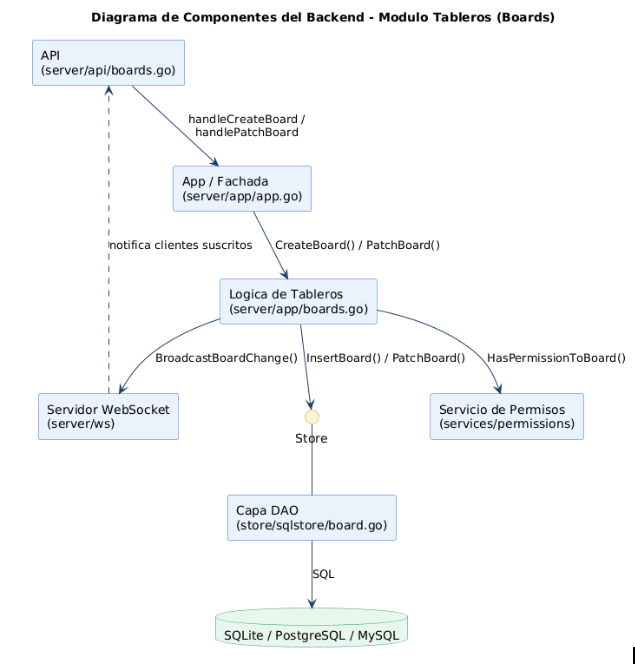
\includegraphics[width=\columnwidth]{../../docs/images/img3.png}
\caption{Componentes verificados por el pipeline de GitHub Actions.}
\label{fig:github_actions_pipeline}
\end{figure}
\vspace{\baselineskip}

% ----------------------------------------------------------------------------
% Results and Discussion
% ----------------------------------------------------------------------------
\section{Resultados y discusión}

% --- Subsection: General Summary ---
\subsection{Resumen general}
La principal semejanza entre los niveles fue el uso de los mismos dominios: autenticación, tableros, tarjetas y permisos. La diferencia estuvo en lo observado. Las pruebas unitarias aislaron condiciones de error; las funcionales mostraron el comportamiento disponible para el usuario; las de integración verificaron efectos entre capas; y las de sistema recorrieron el producto desplegado. Los 56 casos de integración y los dos E2E aprobaron, mientras la ejecución funcional mostró 17 casos no exitosos y 9 pendientes.

La comparación también mostró que un nivel puede revelar una limitación que otro no observa. Un mock confirma que el manejador reacciona ante un error del Store, pero no descubre una migración incompatible. Una integración confirma la escritura, pero no muestra si el control resulta visible o conserva el foco. Un E2E comprueba el recorrido principal, aunque puede omitir clases inválidas que resultan más económicas de probar en la API. Por ello, aumentar únicamente la cantidad de E2E no habría producido la misma cobertura de riesgos.
\vspace{\baselineskip}

% --- Subsection: Coverage Achieved ---
\subsection{Cobertura alcanzada}
La cobertura global fue 71.4\%. Por tanto, no se alcanzó el criterio de 85\%. Este resultado no contradice el éxito de suites concretas: una suite puede aprobar y dejar rutas sin ejecutar. El porcentaje sirvió para localizar deuda, no para sustituir la revisión de requisitos ni los resultados de integración.

La lectura del porcentaje exigió mantener estable el alcance de medición. En el backend, el perfil de Go registra las sentencias instrumentadas de los paquetes seleccionados; en el frontend, Jest contabiliza sentencias, ramas, funciones y líneas. SonarQube reúne los reportes mediante su propio modelo y presenta un valor global. Por ello, no se calculó un promedio simple entre el porcentaje de Go y el de Jest: ambos conjuntos contienen cantidades distintas de código y un promedio sin ponderación podría elevar o reducir artificialmente el resultado. El 71.4\% presentado corresponde al análisis global del repositorio y se conservó como cifra principal.

También se distinguió entre exclusión técnica y exclusión motivada por el resultado. Es razonable retirar archivos generados, declaraciones sin comportamiento ejecutable o mocks creados por herramientas, siempre que la regla se documente antes de observar el porcentaje. En cambio, excluir un manejador, servicio o componente porque no fue cubierto cambia el denominador y no mejora las pruebas. Esta diferencia fue importante durante el trabajo: el objetivo no consistió en producir una cifra favorable, sino en saber qué parte del código productivo todavía no había sido ejercitada.

La distancia de 13.6 puntos porcentuales respecto del umbral representa trabajo pendiente distribuido, no una cantidad fija de casos. Una prueba puede ejecutar muchas sentencias lineales y aportar poco sobre decisiones; otra puede cubrir una sola rama crítica, como la denegación de acceso a un tablero ajeno. En consecuencia, la ampliación debe priorizar primero archivos con baja cobertura y responsabilidad de negocio, y después diseñar casos para sus ramas de éxito, validación y error. Esa estrategia permite que el incremento sea defendible y, al mismo tiempo, reduzca riesgos concretos.
\vspace{\baselineskip}

% --- Subsection: Defects Found ---
\subsection{Defectos encontrados}
Los casos no exitosos señalaron problemas en autenticación, compartición, restauración y suscripciones. Algunos fueron bloqueos funcionales y otros diferencias entre el catálogo esperado, la edición evaluada y el entorno de un solo usuario. Se evitó clasificar automáticamente los diecisiete como defectos confirmados. Cada uno requiere reproducción, contraste con la versión y determinación de causa antes de registrarse como incidente del producto.
\vspace{\baselineskip}

% --- Subsection: Limitations ---
\subsection{Limitaciones}
El trabajo estuvo limitado por el tiempo, el entorno de un usuario, la dependencia de Docker para Cypress en Windows y la falta de datos suficientes para fijar un SLA. Nueve casos funcionales no pudieron ejecutarse. Las pruebas de sistema cubrieron dos atributos y modelos reducidos; no incluyeron carga, disponibilidad prolongada, pentesting ni evaluación de accesibilidad con participantes. Focalboard tampoco se encuentra mantenido actualmente en su repositorio comunitario, lo que condiciona la corrección de deuda heredada \cite{focalboardRepo}.

Los resultados de usabilidad deben entenderse dentro de ese alcance. Cypress verificó que un usuario pudiera crear un tablero y reconocer el efecto esperado en la interfaz, pero no midió aprendizaje, satisfacción ni tiempo de tarea con una muestra de participantes. Del mismo modo, el escenario de seguridad comprobó controles de autenticación y acceso observables durante el recorrido automatizado; no reemplaza un análisis de vulnerabilidades, una revisión criptográfica ni una prueba de penetración. Se evaluaron manifestaciones concretas de dos atributos, no la totalidad de cada atributo de calidad.

La ejecución funcional también tuvo una limitación de comparabilidad. Algunos casos provenían de un catálogo amplio y encontraron diferencias de edición o funciones que requerían más de un usuario. Por esa razón, un resultado no exitoso se conservó como evidencia de ejecución, pero no se convirtió directamente en defecto. Esta precaución evita mezclar tres situaciones distintas: una falla reproducible del producto, una precondición que el entorno no satisface y una expectativa que corresponde a otra versión. La clasificación definitiva necesita repetir el caso con versión, datos y precondiciones controlados.

Finalmente, los tiempos de los jobs de GitHub Actions muestran duración de la automatización, pero no constituyen una prueba de desempeño de Focalboard. En esos tiempos influyen la asignación del runner, la descarga de dependencias, la construcción de imágenes y el almacenamiento de artefactos. Para evaluar desempeño sería necesario separar preparación y medición, estabilizar los datos, repetir cada carga y reportar latencia, rendimiento y dispersión. Esa prueba quedó fuera de los dos atributos seleccionados.
\vspace{\baselineskip}

% ----------------------------------------------------------------------------
% Conclusions
% ----------------------------------------------------------------------------
\section{Conclusiones}
En este trabajo se logró establecer una estrategia reproducible para probar Focalboard en cuatro niveles. La trazabilidad permitió relacionar requisitos, casos y componentes. Se ejecutaron 97 casos funcionales, 56 casos de integración y dos escenarios E2E de sistema. La integración y los escenarios de seguridad y usabilidad aprobaron; la evaluación funcional encontró resultados que requieren revisión adicional.

El principal hallazgo es que los niveles se complementan. Los mocks facilitaron provocar errores, pero solo la integración confirmó la persistencia y los permisos en conjunto; Cypress comprobó recorridos completos, pero no sustituyó las pruebas negativas de API. La cobertura global de 71.4\% quedó por debajo del objetivo. Por ello, el resultado más útil no fue declarar un cumplimiento inexistente, sino identificar las rutas y condiciones que todavía necesitan pruebas.

La automatización dejó además una base verificable para continuar el trabajo. Los tres workflows académicos separan cobertura unitaria, integración de APIs críticas y sistema E2E, mientras SonarQube mantiene una lectura transversal de calidad. Esta separación hace visible qué evidencia produce cada job y evita presentar como equivalentes una suite aprobada y un umbral de cobertura cumplido. En la exposición final, el cumplimiento puede sustentarse con los casos ejecutados, los artefactos del pipeline y los resultados del Quality Gate, incluidos aquellos que permanecen por debajo de la meta.
\vspace{\baselineskip}

% ----------------------------------------------------------------------------
% Future Work
% ----------------------------------------------------------------------------
\section{Trabajos futuros}
Como trabajo futuro se propone completar los nueve casos funcionales pendientes en un entorno multiusuario, reproducir y clasificar los diecisiete resultados no exitosos y ampliar las pruebas unitarias sobre módulos de baja cobertura. También se propone añadir pruebas de valores límite para credenciales y títulos, automatizar más escenarios Cypress, medir rendimiento con una línea base repetible e incorporar análisis de accesibilidad y seguridad especializado. Finalmente, conviene configurar el Quality Gate para vigilar código nuevo sin ocultar la cobertura histórica y conservar tendencias por ejecución.
\vspace{\baselineskip}

% ----------------------------------------------------------------------------
% References
% ----------------------------------------------------------------------------
\begin{thebibliography}{00}
\bibitem{focalboardRepo}
Mattermost Community, ``Focalboard: Open source project management tool,'' GitHub repository, 2024. [Online]. Available: \url{https://github.com/mattermost-community/focalboard}. Accessed: Jul. 18, 2026.

\bibitem{iso25010}
ISO/IEC, ``ISO/IEC 25010:2023 Systems and software engineering---Systems and software Quality Requirements and Evaluation (SQuaRE)---Product quality model,'' 2023. [Online]. Available: \url{https://www.iso.org/standard/78176.html}.

\bibitem{goCoverage}
The Go Authors, ``Coverage profiling support for integration tests,'' Go Documentation. [Online]. Available: \url{https://go.dev/doc/build-cover}. Accessed: Jul. 18, 2026.

\bibitem{jestDocs}
OpenJS Foundation, ``Configuring Jest: collectCoverageFrom,'' Jest Documentation. [Online]. Available: \url{https://jestjs.io/docs/configuration#collectcoveragefrom-array}. Accessed: Jul. 18, 2026.

\bibitem{cypressDocs}
Cypress.io, ``End-to-end testing: your first test with Cypress,'' Cypress Documentation. [Online]. Available: \url{https://docs.cypress.io/app/end-to-end-testing/writing-your-first-end-to-end-test}. Accessed: Jul. 18, 2026.

\bibitem{githubActions}
GitHub, ``Continuous integration with GitHub Actions,'' GitHub Documentation. [Online]. Available: \url{https://docs.github.com/en/actions/get-started/continuous-integration}. Accessed: Jul. 18, 2026.

\bibitem{sonarGates}
SonarSource, ``Quality gates,'' SonarQube Cloud Documentation. [Online]. Available: \url{https://docs.sonarsource.com/sonarqube-cloud/standards/quality-gates}. Accessed: Jul. 18, 2026.

\bibitem{ciReview}
E. Soares, G. Sizilio, J. Santos, D. A. da Costa, and U. Kulesza, ``The effects of continuous integration on software development: a systematic literature review,'' \textit{Empirical Software Engineering}, vol. 27, art. no. 78, 2022, doi: \href{https://doi.org/10.1007/s10664-021-10114-1}{10.1007/s10664-021-10114-1}.
\end{thebibliography}

\end{document}
